\documentclass[preprint,12pt]{elsarticle}
\usepackage[T1]{fontenc}
\usepackage[utf8]{inputenc}
\usepackage[brazil]{babel}
\usepackage{amsmath,amssymb,booktabs,graphicx,xurl,placeins}
\usepackage[hidelinks]{hyperref}
\setlength{\emergencystretch}{2em}
\renewcommand{\floatpagefraction}{0.8}
\renewcommand{\topfraction}{0.9}
\renewcommand{\textfraction}{0.1}
\journal{Supply Chain Analytics -- manuscrito de trabalho em português}
\begin{document}
\begin{frontmatter}
\title{AIPE: uma metodologia modular para seleção contextual de políticas de reposição}
\author[ufal]{Matheus Inácio Batista Santos}
\affiliation[ufal]{organization={Instituto de Computação, Universidade Federal de Alagoas},country={Brasil}}
\begin{abstract}
A heterogeneidade da demanda motiva selecionar políticas de reposição por contexto, mas a diversidade de vencedoras não assegura recomendações melhores. Propomos o Adaptive Inventory Policy Engine (AIPE), uma metodologia modular que vincula representação do contexto, evidência operacional, seleção e avaliação. Seu Policy Selection Engine (PSE) associa perfis a famílias de políticas ou estima recomendações por série, com uma regra explícita para substituir ou conservar a referência. Avaliamos sete candidatas em duas aplicações separadas. Na Bahia, 145 séries em duas origens totalizam 4.350 ajustes; a seleção por perfil aumenta o atendimento em 3,89 pontos percentuais e o custo em 1,93\% frente à referência global. No piloto Walmart M5, 30 séries de dez lojas em três origens totalizam 1.350 ajustes. O preditivo por classe apresenta custo 13,9\% maior e atendimento 4,11 pontos inferior. Uma extensão exploratória por consequências previstas, com recuo à referência, reduz custo em 1,56\% e aumenta atendimento em 0,27 ponto; apenas três de 90 decisões mudam, e uma série concentra cerca de 92\% da economia. A contribuição é um procedimento que torna verificáveis a recomendação, sua utilidade incremental e as causas das perdas. Os resultados delimitam as instanciações avaliadas; calibrações específicas e desenvolvimento no piloto exigem confirmação independente.

\end{abstract}
\begin{keyword}
Inventory methodology \sep Modular decision support \sep Policy selection \sep Demand heterogeneity \sep Service level
\end{keyword}
\end{frontmatter}

\section{Introdução}
Selecionar uma política de reposição para cada combinação de loja e produto exige conciliar custo e atendimento sob demandas heterogêneas. Vendas frequentes, intervalos sem demanda e picos ocasionais podem favorecer regras diferentes. A vantagem de contextualizar a escolha, porém, depende de reconhecer essas diferenças antes da decisão e convertê-las em resultados operacionais posteriores \cite{Axsater2006InventoryControl}.

A escolha da família de política constitui uma decisão distinta da calibração de seus parâmetros. Uma referência global pode usar a mesma família em toda a rede e ainda ajustar lotes e limiares ao histórico de cada série. A seleção de algoritmos fornece uma formulação para ir além dessa referência: características da instância orientam a escolha de um método de um portfólio \cite{rice1976,Kotthoff2014AlgorithmSelection}. No inventário, essa escolha precisa considerar tanto o custo quanto a viabilidade do atendimento.

O desafio é transformar evidência comparativa em uma recomendação justificável. Identificar a melhor candidata após observar o teste informa o potencial do portfólio, mas não demonstra que um seletor consiga antecipá-la. Além disso, uma recomendação pode falhar porque escolheu mal, porque nenhuma candidata atende ao alvo ou porque o sistema não permite atendê-lo nas condições iniciais. Cada situação exige uma intervenção diferente.

Propomos o \textit{Adaptive Inventory Policy Engine} (AIPE), uma metodologia modular para organizar essa decisão. O procedimento especifica o problema, representa o contexto, constrói uma matriz comparável de consequências, recomenda pelo \textit{Policy Selection Engine} (PSE) e avalia a escolha em dados reservados. O PSE admite associação por perfil ou estimação por série. Uma regra de intervenção explicita quando a candidata substitui a referência. Contratos de entrada, saída e informação permitem substituir métodos e reavaliar suas consequências mantendo o problema de decisão definido.

A contribuição metodológica compreende a articulação dessas etapas, a decisão explícita de intervenção e o diagnóstico das perdas. Os controladores e seletores são instanciações usadas para examinar o procedimento. A avaliação distingue sua execução modular de sua utilidade: a primeira requer interfaces compatíveis; a segunda requer benefício em custo e serviço frente à referência. Os antecedentes de classificação de inventário e seleção de algoritmos delimitam o posicionamento apresentado na seção seguinte.

As aplicações usam vendas de uma rede varejista brasileira e um piloto da base pública Walmart M5. A Bahia oferece heterogeneidade empresarial observada; o M5 permite examinar seletores preditivos em um referencial público. As consequências são simuladas, e as bases mantêm custos, populações e calibrações identificados separadamente. A análise inclui ganhos, deteriorações e concentração dos benefícios. As tabelas reportam matrizes auditadas; a avaliação ampliada em andamento permanece fora das conclusões quantitativas.

\section{Trabalhos relacionados}
O intervalo médio entre demandas (\textit{average demand interval}, ADI) e o coeficiente de variação (CV) fundamentam a classificação ADI--CV$^2$, em que CV$^2$ é o quadrado do coeficiente. Essa classificação organiza padrões de frequência e tamanho da demanda \cite{syntetos2005}. Entretanto, classes estatísticas não determinam sozinhas a melhor reposição: custos, prazo, estoque inicial e atendimento também importam. Mohammaditabar et al.\ \cite{Mohammaditabar2012Integrated} integram classificação e escolha de políticas; Sheikh-Zadeh et al.\ \cite{SheikhZadeh2021PBIC} propõem classificação orientada ao desempenho em sistemas de múltiplos itens e escalões. Esses antecedentes fundamentam a metodologia e impedem reivindicar prioridade na integração entre classificação e inventário. Seus métodos não foram reproduzidos como comparadores.

Na literatura da revista, Tadayonrad e Ndiaye \cite{sca_f81ad2b3e023} aproximam previsão e consequências operacionais. Theunissen et al.\ \cite{sca_c5c06dcbc9e5} discutem a informação decisória preservada pela classificação. Essa perspectiva orienta nossa avaliação: reconhecer um perfil ou acertar o nome de uma política só tem utilidade se melhorar a decisão. Não implementamos o método topológico desses autores.

Zabraoui et al.\ \cite{sca_27e994c54848} comparam algoritmos de inventário e combinações de busca genética e aprendizado por reforço com dados M5. A combinação de algoritmo genético (\textit{genetic algorithm}, GA) e rede Q profunda (\textit{deep Q-network}, DQN), denominada GA--DQN, integra nosso portfólio, com seus componentes como controles, sem ser apresentada como contribuição algorítmica. Granularidade, filtros, custos e implementação local impedem uma reprodução exata de seu ranking.

Políticas limitadas de estoque-base oferecem outra referência para vendas perdidas \cite{Xin2021CappedBaseStock}. Suas propriedades teóricas não garantem desempenho para nossa calibração. Os resultados de reforço também dependem do estado, da recompensa e do orçamento \cite{Boute2022DRLInventoryRoadmap}. O AIPE separa essas implementações da escolha entre candidatas. A avaliação do seletor precisa, ainda, separar desenvolvimento e teste para evitar otimismo após escolher configurações \cite{CawleyTalbot2010}.

Francuz e Bányai \cite{FrancuzBanyai2026Selection} integram escolha de família e parâmetros em otimização multiobjetivo, usando aprendizado para aproximar o simulador. A aplicação tem demanda sintética sazonal e pedidos pendentes. Aprendizado orientado à consequência \cite{ElmachtoubGrigas2022SPO}, predição com rejeição \cite{GeifmanElYaniv2019SelectiveNet} e recuo à referência em aprendizado por reforço (\textit{reinforcement learning}, RL) \cite{Laroche2019SPIBB} também possuem antecedentes. O AIPE articula esses fundamentos na seleção de famílias de reposição; a revisão não demonstra ineditismo universal dessa articulação nem transfere garantias teóricas para o ambiente avaliado.

\section{AIPE: metodologia modular}
\subsection{Objeto e procedimento}
O AIPE organiza a escolha de uma família de reposição para a série loja--produto a partir da informação disponível antes da decisão. A aplicação começa pela definição de históricos e contexto, portfólio, ambiente de estoque, objetivo operacional e desenho de avaliação. Ao final, produz uma recomendação acompanhada da referência, dos parâmetros de aplicação, do suporte da escolha e da identificação da configuração. Quando nenhuma candidata é viável, o registro conserva essa condição mesmo que uma contingência permita emitir a recomendação.

O procedimento tem cinco etapas: (1) especificar unidade, ambiente, objetivo e referência; (2) preparar históricos e representar o contexto; (3) calibrar candidatas e construir evidência de validação; (4) recomendar pelo PSE e aplicar a regra de intervenção; (5) avaliar em dados reservados e diagnosticar perdas. A Figura~\ref{fig:aipe} sintetiza a motivação; a Tabela~\ref{tab:modules} explicita os contratos metodológicos. São responsabilidades do procedimento, não nomes de funções de uma interface de programação universal já disponibilizada.

\begin{figure}[htbp]\centering
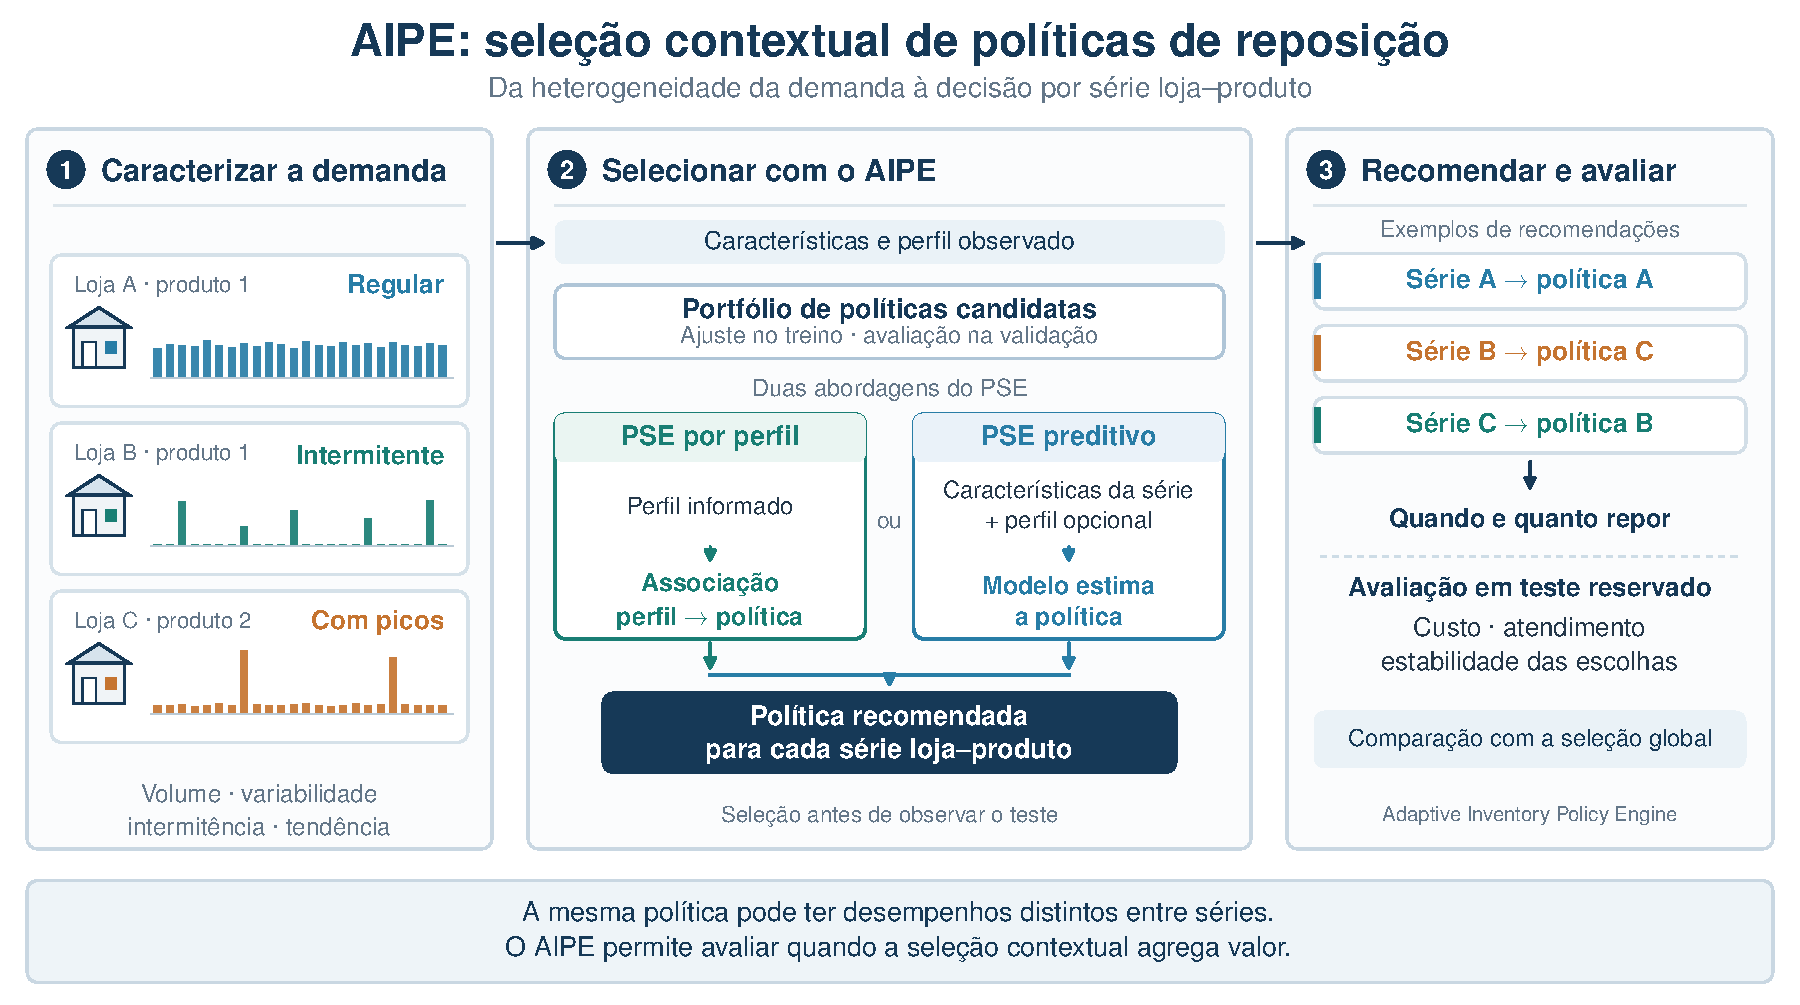
\includegraphics[width=\linewidth]{figures/aipe_conceito_v2_ptbr.pdf}
\caption{AIPE: o contexto orienta a seleção de políticas. O PSE associa um perfil informado a uma família ou estima uma recomendação por série. Famílias A/B/C são ilustrativas; o benefício é avaliado operacionalmente.}\label{fig:aipe}
\end{figure}

\begin{table}[htbp]\centering\small
\caption{Contratos dos módulos do AIPE. Trocar o método preserva a responsabilidade e as restrições de informação.}\label{tab:modules}
\begin{tabular}{@{}p{2.4cm}p{4.0cm}p{4.8cm}@{}}\toprule
Módulo & Entrada e saída & Contrato e instanciação avaliada\\\midrule
Especificação & Requisitos $\to$ cenário e regra & Definir custo, serviço e referência; aqui, vendas perdidas e prazo fixo\\
Contexto & Histórico $\to$ características ou perfil & Usar informação anterior à escolha; descritores e regras fixas\\
Evidência & Cenário e candidatas $\to$ consequências & Ajustar no treino e medir na validação; sete candidatas clássicas, GA e RL\\
PSE & Contexto e evidência $\to$ recomendação & Preservar objetivo e corte temporal; perfil, classe vencedora ou consequências previstas\\
Avaliação & Recomendação fixada $\to$ comparação e diagnóstico & Teste reservado, referência competitiva e perdas identificáveis\\\bottomrule
\end{tabular}\end{table}

\subsection{Substituição dos métodos e decisão de intervenção}
A modularidade significa substituir um método dentro de uma responsabilidade sem alterar o significado dos demais resultados. Um controlador recebe o estado admitido e produz pedido válido; um descritor usa o histórico disponível; um seletor retorna uma família pertencente ao portfólio. Custos, serviço, cronologia e identidade das unidades devem permanecer compatíveis. Métodos com ações ou informações diferentes exigem adaptação e nova verificação, não apenas troca de nome.

Seja $\Pi$ o portfólio, $x_i$ a descrição do treino e $g_i$ o perfil. O PSE por perfil recomenda $m(g_i)$; o preditivo recomenda $f(x_i,g_i)$ ou $f(x_i)$. Ele pode aprender um rótulo ou estimar consequências por candidata. A referência global mantém a família, com parâmetros calibrados individualmente. A regra de intervenção escolhe entre candidata $\widehat\pi_i$ e referência $\pi_i^{\mathrm{ref}}$:
\[
 \pi_i^{\mathrm{AIPE}}=
 \begin{cases}\widehat\pi_i,&a_i=1,\\\pi_i^{\mathrm{ref}},&a_i=0.\end{cases}
\]
A implementação direta admite a recomendação sem recuo; a conservadora exige evidência de benefício. Critérios são definidos no desenvolvimento. Confiança de classe e serviço previsto não garantem atendimento realizado.

A avaliação exercita a substituição de controladores e seletores, mantendo a representação de contexto e o simulador. Todas as candidatas são ajustadas nas unidades de teste para medir as consequências das recomendações e construir os oráculos. Essa despesa experimental difere do uso pretendido, em que evidências anteriores orientariam a família a calibrar; eventual economia computacional de implantação requer avaliação própria. A adaptação aqui estudada é a escolha por contexto e sua reavaliação documentada, com alcance restrito às interfaces exercitadas.

A implementação preserva esses contratos ao ajustar imputação e codificação dentro de cada partição de treinamento e exigir uma matriz completa de políticas, sementes e blocos. Recomendações, referências e intervenções são registradas antes da pontuação do teste. O reaproveitamento de ajustes depende de auditoria da equivalência de dados, configuração e código.

\subsection{Custo, serviço e escolha}
Para demanda $d_t$, quantidade atendida $v_t$, saldo $I_t$ e pedido $q_t$, avaliamos
\begin{equation}
 C=\sum_t[hI_t+p(d_t-v_t)+K\mathbf1(q_t>0)+cq_t],
 \qquad F=\frac{\sum_t v_t}{\sum_t d_t}.
 \label{eq:metrics}
\end{equation}
O atendimento $F$ é \textit{fill rate}, não probabilidade de ciclo sem falta. Diferenças entre taxas de atendimento são expressas em pontos percentuais (p.p.). Com demanda zero, permanece indefinido; o custo continua contabilizado. Na instanciação, usamos $h=1$, $p=5$, $K=50$ e $c=0{,}5$, sem equivalência monetária calibrada.

Na validação $A$, a regra global minimiza $\bar C_{\pi,A}$ entre candidatas com $\bar F_{\pi,A}\geq\alpha$, com $\alpha=0{,}70$. O PSE por perfil aplica essa regra a cada grupo $A_g$. Casos sem demanda não entram na média de serviço. Sem candidata viável, escolhe-se maior serviço e menor custo, registrando contingência. Perfis sem suporte usam a global. Na Bahia, empate no custo viável prefere maior serviço e depois identificador; no M5, prefere identificador. Contingências empatadas em serviço preferem menor custo. Essas convenções são preservadas por base e registradas no código.

O rótulo supervisionado aplica a restrição à própria série de validação: menor custo viável ou, sem viável, maior serviço e menor custo. Se todas as opções têm serviço indefinido, utiliza menor custo e mantém a marcação de demanda zero. Classificador e seletores agregados não impõem a mesma distribuição da restrição. Incluímos a moda dos rótulos como controle para não atribuir toda diferença à capacidade preditiva.

\subsection{Características e perfis}
O preditivo recebe 17 descritores: ADI, CV$^2$, intermitência, proporção de zeros, maior e média das sequências de zeros, \textit{burstiness}, assimetria, curtose, entropia, tendência, autocorrelação, média, desvio-padrão, CV, extensão e número de ciclos positivos. O perfil categórico deriva desses descritores, sem constituir informação independente.

Os perfis usam regras ordenadas e fixas: esparso (ADI $\geq1{,}32$, CV$^2\geq0{,}49$, sequência de zeros $\geq5$); volatilidade/sazonalidade (autocorrelação $\geq0{,}25$ ou burstiness $\geq0{,}30$); tendência instável (tendência absoluta $\geq0{,}05$ ou entropia $\geq2$); baixo volume estável (média $\leq2$ e CV$^2<0{,}49$); e venda frequente (ADI $<1{,}32$). A primeira regra satisfeita define o perfil; o residual é esparso. ADI é $n/\max(n_+,1)$ e CV$^2$ inclui zeros, diferindo da taxonomia original baseada em tamanhos positivos. Os nomes são heurísticos.

Burstiness compara o desvio e a média dos intervalos positivos pela razão de sua diferença e soma, com regularização numérica. Tendência é a inclinação ajustada por mínimos quadrados ordinários dividida pela média; entropia usa dez classes de mesma largura. A autocorrelação na defasagem 17 recebe zero com até 18 ciclos ou variância desprezível. Essa convenção denota estimativa indisponível, não ausência de sazonalidade; com 23 ciclos, há somente seis pares.

\section{Desenho experimental}
A avaliação examina três questões: a seleção por perfil melhora o compromisso entre custo e atendimento; a estimação por série acrescenta valor à referência; e as perdas observadas podem ser atribuídas à seleção, ao portfólio ou à viabilidade física? A Bahia investiga a primeira questão; o piloto M5 reúne as comparações preditivas e os diagnósticos. A comparação por consequências reutiliza sua matriz para examinar outra implementação do PSE.
\subsection{Bases e unidades de análise}
A Tabela~\ref{tab:datasets} distingue as avaliações. Na Bahia, transações complementares são somadas por loja, produto e ciclo; ciclos sem venda recebem zero. A coorte retrospectiva contém 145 séries, 115 lojas e nove produtos. Os 38 ciclos disponíveis, de 202301 a 202504, são unidades comerciais da fonte, não meses.

O M5 é uma fonte pública de vendas associada a uma competição de previsão \cite{Makridakis2022M5Accuracy}. Os códigos de lojas preservados do M5 combinam o estado e um identificador local: CA designa Califórnia, TX designa Texas e WI designa Wisconsin; por exemplo, CA\_2 identifica uma loja da Califórnia. O piloto sorteia 30 séries da categoria de alimentos (\texttt{FOODS}), três por loja nas dez lojas. Na primeira origem, o volume médio do treino define três estratos por loja, com uma escolha em cada estrato e semente 20261015. As séries são mantidas nas três origens. Usamos ciclos completos de 21 dias, sem remover picos por regras baseadas no intervalo interquartil.

\begin{table}[htbp]\centering\small
\caption{Matrizes completas analisadas. Casos série--origem e sementes não são séries independentes.}\label{tab:datasets}
\begin{tabular}{@{}lrr@{}}\toprule
Dimensão & Bahia & Piloto M5\\\midrule
Séries / lojas & 145 / 115 & 30 / 10\\
Origens de treino (ciclos) & 17 e 23 & 50, 64 e 78\\
Validação / teste por origem & 7 / 7 & 7 / 7\\
Casos série--origem & 290 & 90\\
Ajustes de políticas & 4.350 & 1.350\\
Testes sem demanda & 7 & 4\\
Seletores & Global e por perfil & Global, por perfil e preditivo\\\bottomrule
\end{tabular}\end{table}

A elegibilidade exige três ciclos positivos no prefixo. O sorteio M5 usa 885 séries elegíveis na primeira origem de uma coorte histórica de 2.408 identificadores. Não representa todas as FOODS nem séries elegíveis somente depois. O recorte é inspirado no contexto de Zabraoui et al., sem afirmar identidade com sua amostra. A continuidade da rodada maior não fornece ainda conclusões deste artigo.

\subsection{Simulador, portfólio e calibração}
O prazo exato é de dois ciclos. A política observa o estado anterior ao recebimento; entregas chegam antes da demanda. Quantidades podem ser fracionárias. Faltas são vendas perdidas, sem pedidos pendentes. Manutenção incide no saldo após demanda e o pedido é custeado na emissão, sem crédito terminal.

Validação e teste começam em estados comuns às candidatas, produzidos por uma referência de lote econômico de compra (\textit{economic order quantity}, EOQ): seis ciclos passados aquecem o sistema, e sua trajetória na validação determina estoque e pipeline do teste. Esses estados usam o passado, mas não representam a continuação particular de cada candidata. Escalas são calculadas no treino.

O portfólio contém EOQCycle, sSCycle, CappedBaseStock, GA, otimização proximal de políticas (\textit{proximal policy optimization}, PPO), GA--DQN e DQN. EOQCycle usa lote $\max(1,\sqrt{2\mu K/h})$ e ponto de pedido $2\mu+1{,}28\sigma\sqrt2$; sSCycle repõe até o ponto acrescido do lote. CappedBaseStock limita a quantidade da reposição até um alvo e calibra alvo e teto em grade $20\times12$. GA ajusta gatilho, lote e proteção com população 100 e 50 gerações. DQN usa Double DQN dueling; PPO usa otimização proximal. Ambos têm duas camadas de 64 unidades, 20 ações e no mínimo 20 mil transições, arredondadas ao episódio completo. GA--DQN acrescenta busca genética e mil demonstrações, mantendo gatilho e piso iguais nas demonstrações, treino e inferência.

Os quatro métodos estocásticos usam sementes 11, 29 e 47; as três referências determinísticas têm um ajuste. As sementes são promediadas antes da avaliação por caso. O híbrido tem esforço superior ao DQN, sem equivalência de orçamento. A calibração pode penalizar déficit de serviço. Na matriz Bahia reportada, CappedBaseStock também penaliza frequência de ruptura e amplificação dos pedidos com pesos unitários; no M5, ambos os pesos são zero. Essa diferença impede atribuir contrastes entre bases somente à demanda. Cada matriz e código arquivado identificam a instanciação avaliada.

\subsection{Avaliação e desenvolvimento do piloto}
Em cada origem, uma loja inteira fica fora do conjunto que define a escolha. O PSE usa a validação das demais lojas e recomenda para o teste da loja reservada. Controladores continuam calibrados no histórico da própria série: avaliamos transferência do seletor com histórico disponível, não implantação sem dados prévios.

No M5, XGBoost tem 200 árvores, profundidade três, taxa 0,05, sem subamostragem e com semente fixa. Imputação, codificação categórica e classes são ajustadas dentro de cada fold. Classes raras não são removidas; treinos de classe única usam classificador constante. Cada treinamento reúne 27 exemplos. A ablação sem perfil mantém os demais componentes. Não se usam origens posteriores para recomendar em uma origem anterior.

Uma implementação com recuo usa o PSE por perfil se o maior escore de classe for inferior a 0,60 ou a classe prevista tiver menos de três exemplos de treino. Não há busca de limiares no teste, mas a motivação veio dos resultados observados. Seu desempenho é exploratório, e o piloto passa a ser conjunto de desenvolvimento \cite{CawleyTalbot2010}. O escore não é probabilidade calibrada de viabilidade.

A comparação reduzida adicional reutiliza a matriz M5 e substitui a implementação do PSE. Duas florestas ExtraTrees estimam custo e serviço por candidata: 64 árvores, profundidade quatro, mínimo de três observações por folha e semente fixa. Custo usa $\log(1+C)$, transformado de volta; serviço exclui alvos indefinidos. A seleção direta escolhe o menor custo previsto viável; sem viável, prioriza serviço e depois custo.

A variante com recuo à global exige serviço previsto $\geq0{,}70$, não inferior ao previsto da referência, e economia acima de uma margem em $\{0;0{,}02;0{,}05;0{,}10;\infty\}$. A margem minimiza custo em validação interna por loja, sujeita a serviço médio não inferior à referência. Cada origem exclui uma loja externa; dentro das nove restantes, ajusta em oito e valida na nona. A margem é fixada antes da recomendação externa. Um classificador ExtraTrees com a mesma regularização controla a aprendizagem por rótulo, e uma ablação retira perfil do seletor por consequências sem recuo. Recomendações são gravadas antes da pontuação do teste, mas o piloto já orientou o desenvolvimento: a comparação permanece exploratória.

Na Bahia, os testes compartilham um ciclo; no M5, ocupam os ciclos 58--64, 72--78 e 86--92, sem sobreposição. Origens repetem séries. Intervalos exploratórios usam bootstrap pareado por loja, preservando séries e origens: 5.000 sorteios na Bahia, 2.000 na comparação de perfil e classe no M5 e 5.000 na comparação por consequências. Seletores e controladores permanecem fixos; a incerteza é condicional, sem novos treinamentos. Dez lojas do piloto limitam sua precisão.

\subsection{Avaliação unificada e alcance dos resultados}
O protocolo ampliado avalia as mesmas variantes do PSE separadamente na Bahia e no recorte M5, com identificação das matrizes e dos procedimentos que geraram cada resultado. A avaliação ampliada usa cinco grupos internos de lojas para escolher a margem de recuo; a loja externa permanece excluída em cada origem. No piloto reduzido reportado, a escolha interna excluiu uma loja por vez. O novo desenho reduz o número de ajustes internos, mas pode alterar as recomendações; seus resultados não substituem os do piloto antes de conferência.

A calibração unificada da CappedBaseStock usa pesos zero para ruptura e amplificação em ambas as bases. Somente checkpoints afetados por essa diferença precisam ser refeitos; os demais exigem equivalência de código, configuração e dados. A aplicação brasileira conserva as 145 séries e amplia a avaliação dos seletores. O M5 conserva 2.408 identificadores históricos, com 885, 2.033 e 2.408 elegíveis nas três origens; não representa todas as FOODS. O resumo separará as séries usadas no piloto das demais, sem tratar essa separação como prova de independência. As métricas apresentadas a seguir continuam vinculadas às calibrações e validações que efetivamente as produziram.

\subsection{Oráculos e informação perfeita}
O melhor controlador único no teste é um diagnóstico retrospectivo. O oráculo do portfólio escolhe, por série--origem, a candidata de menor custo viável nas médias de teste entre sementes. Essas escolhas não fornecem rótulos ao treinamento. O acerto exige serviço mínimo e empate numérico no menor custo; concordância nominal é informada separadamente.

No M5, um programa linear inteiro misto (\textit{mixed-integer linear programming}, MILP) conhece toda a demanda de teste e otimiza pedidos sob os mesmos custos, prazo e condições iniciais. Quantidades são contínuas; variáveis binárias representam emissão e complementaridade entre saldo e falta. É um ótimo determinístico condicional, não um controlador estocástico implantável. Se 0,70 for fisicamente impossível antes das primeiras entregas, maximiza atendimento e depois minimiza custo. Soluções são reexecutadas no simulador e somente as comprovadamente ótimas recebem essa denominação.

A eficiência de custo é $100C^*/C_{\mathrm{PSE}}$, apenas quando referência e recomendação satisfazem o mesmo critério de serviço; ambos os custos zero equivalem a 100\%. Serviço insuficiente não recebe crédito por custo baixo. A comparação com o MILP usa cada realização de treinamento viável: uma média entre sementes pode satisfazer o alvo sem que todas o satisfaçam. Repetir políticas determinísticas nessa análise não gera novas observações independentes.

\section{Resultados na Bahia: PSE por perfil}
\label{sec:ba2026}
As sete candidatas foram avaliadas em 290 casos série--origem. O custo médio usa todos os casos e o atendimento os 283 com demanda positiva; sete têm serviço indefinido. Somente EOQCycle e sSCycle superam 0,70 em média; nenhuma supera esse alvo no atendimento ponderado pelas unidades demandadas.

\begin{figure}[htbp]\centering
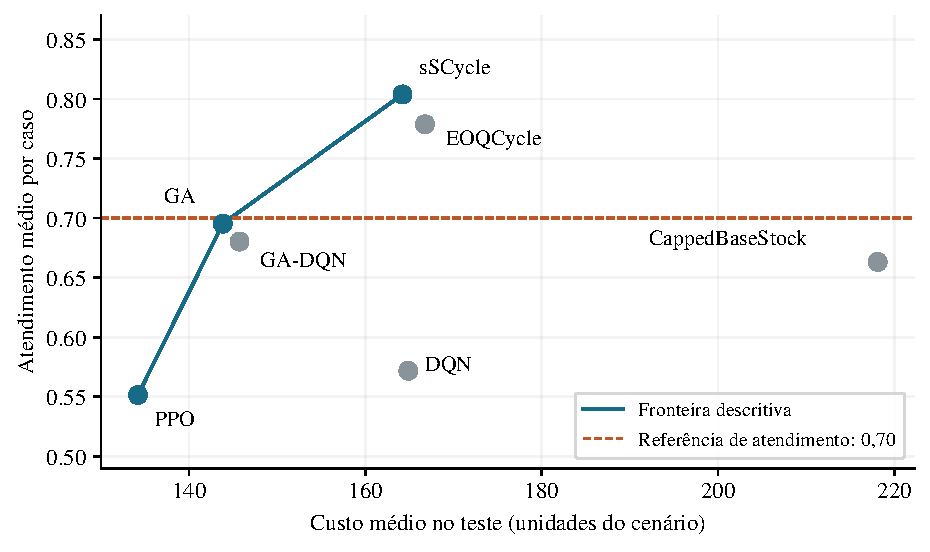
\includegraphics[width=.92\linewidth]{figures/custo_servico.pdf}
\caption{Portfólio na Bahia: custo médio em 290 casos e atendimento em 283 com demanda positiva. A fronteira é retrospectiva e descritiva; não é usada para escolher no teste.}\label{fig:cost_service}
\end{figure}

PPO tem menor custo e menor atendimento. GA--DQN reduz custo em 11,60\% frente ao DQN e eleva atendimento de 0,5718 para 0,6802; frente ao GA, custa 1,32\% mais e atende menos. O híbrido não domina seu componente evolutivo no agregado, e seu esforço adicional impede atribuir o contraste apenas à combinação algorítmica.

\begin{table}[htbp]\centering\small
\caption{Escolha na validação das demais lojas; teste da loja reservada. Custo em 145 casos por linha; atendimento em 144 casos na origem 17 e 139 na origem 23.}\label{tab:ba2026_selection}
\begin{tabular}{@{}llrrr@{}}\toprule
Treino & Seleção & Custo & Atendimento & Abaixo de 0,70\\\midrule
17 ciclos & Global &180,58&0,5711&101\\
17 ciclos & PSE por perfil &186,79&0,6475&82\\
23 ciclos & Global &142,03&0,9073&18\\
23 ciclos & PSE por perfil &142,03&0,9073&18\\\bottomrule
\end{tabular}\end{table}

Na primeira origem, a global escolhe GA em todos os casos. O PSE por perfil escolhe GA em 65, sSCycle em 75 e EOQCycle em cinco. Na segunda, ambos escolhem sSCycle nos 145 casos. A Figura~\ref{fig:profile_choices} localiza essa diferenciação: perfis distintos não implicam recomendações distintas em todo período.

\begin{figure}[htbp]\centering
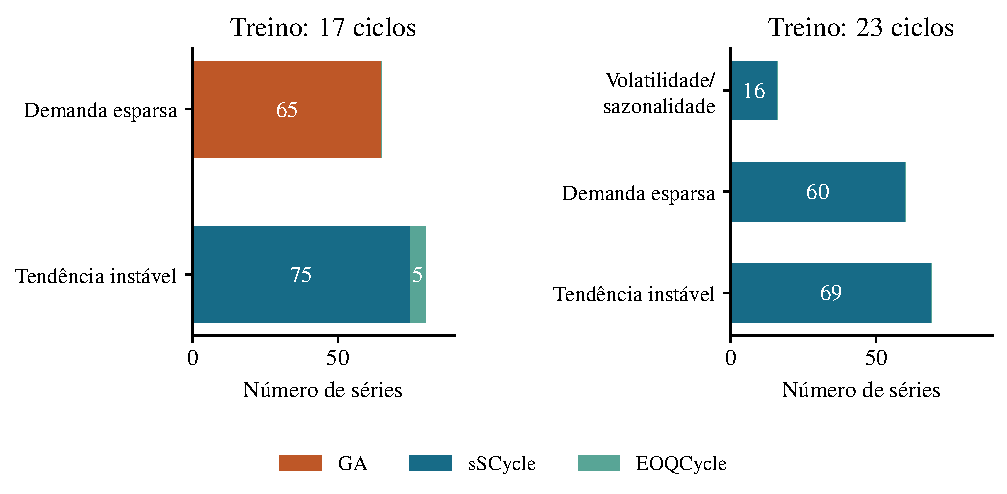
\includegraphics[width=\linewidth]{figures/escolhas_perfil.pdf}
\caption{Escolhas do PSE por perfil na Bahia, com meta 0,70. Há 145 recomendações por origem. A segunda reproduz a seleção global.}\label{fig:profile_choices}
\end{figure}

Reunindo origens, o custo passa de 161,31 para 164,41, aumento de 1,93\%; o atendimento cresce de 0,7362 para 0,7751, diferença de 3,89 pontos percentuais. O ponderado passa de 0,5750 para 0,6395. Casos abaixo de 0,70 diminuem de 119 para 100 entre 283 definidos. O resultado é serviço adicional com custo pontualmente maior, concentrado na primeira origem.

O bootstrap condicional de 115 lojas produz intervalos de 95\% de $[-0{,}32;4{,}16]\%$ para custo e $[2{,}78;5{,}07]$ pontos para atendimento. Incluir zero no intervalo de custo não prova equivalência. Variar o limiar sem recalibrar o portfólio também não preserva o benefício: em 0,80, o PSE por perfil custa mais e atende ligeiramente menos; em 0,85, ambos escolhem sSCycle em todos os casos; em 0,90 e 0,95, todas as escolhas são contingências na validação.
\FloatBarrier

\section{Resultados no M5: duas abordagens do PSE}
\label{sec:m5pse}
\subsection{Custo e atendimento das recomendações}
O piloto completa os 1.350 ajustes das 30 séries em três origens. As recomendações são avaliadas em 90 casos, com atendimento definido em 86. Não são 90 séries independentes. A Tabela~\ref{tab:m5_selectors} inclui dois controles: moda dos rótulos de treino e escolha individual da vencedora de validação. O último examina a transferência temporal do próprio rótulo, sem representar um limite superior para os seletores.

\begin{table}[htbp]\centering\small
\caption{M5: custo em 90 casos; atendimento e contagem de viáveis em 86 com demanda positiva. O recuo é exploratório, desenvolvido após o diagnóstico do piloto.}\label{tab:m5_selectors}
\begin{tabular}{@{}lrrr@{}}\toprule
Seleção & Custo & Atendimento & Casos $\geq0{,}70$\\\midrule
Global &1.086,97&0,7146&47\\
PSE por perfil &1.094,02&0,7091&46\\
PSE preditivo com perfil &1.238,30&0,6735&39\\
PSE preditivo sem perfil &1.238,30&0,6735&39\\
Moda dos rótulos &1.096,65&0,6885&42\\
Individual na validação &1.185,13&0,6838&44\\
Preditivo com recuo &1.087,26&0,6996&46\\\bottomrule
\end{tabular}\end{table}

O preditivo custa 13,9\% mais e atende 4,11 pontos percentuais menos que a global. O contraste desfavorável aparece nas três origens e nos dois perfis. WI\_3 e TX\_2 respondem por 65,4\% da diferença líquida de custo. O PSE por perfil permanece próximo da global: maior custo e serviço ligeiramente menor, sem benefício agregado neste piloto.

\begin{figure}[htbp]\centering
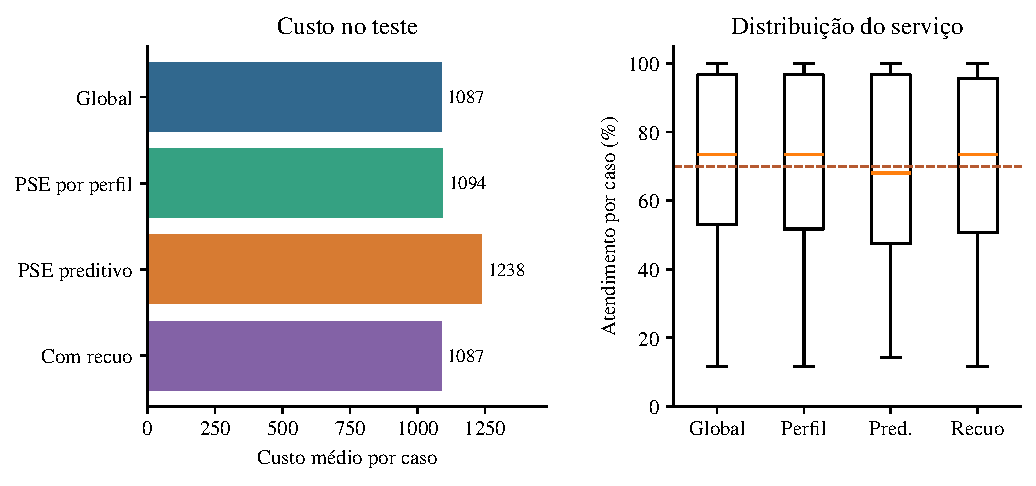
\includegraphics[width=\linewidth]{figures/aipe_m5_comparacao.pdf}
\caption{Piloto M5: custo e atendimento médios são apresentados separadamente. Caixas descrevem o serviço nos 86 casos definidos; linha em 0,70. O recuo foi desenvolvido no piloto, sem confirmação independente.}\label{fig:m5_comparison}
\end{figure}

O recuo é acionado em 62 casos e muda a política em 48. Frente ao preditivo, reduz custo em 12,2\% e aumenta serviço em 2,62 pontos. Frente à global, custa 0,026\% mais e atende 1,49 ponto menos; o atendimento permanece abaixo de 0,70. O intervalo exploratório para a diferença de custo frente à global é $[-39{,}83;39{,}30]$ unidades do cenário; para serviço, $[-2{,}87;-0{,}23]$ pontos. Proximidade de custo não comprova equivalência.

\subsection{O que explica a dificuldade do preditivo?}
Cada fold tem 27 exemplos para até sete classes. O modelo reproduz 100\% dos rótulos do treino, mas somente 19 dos 90 rótulos de validação das lojas excluídas. Dois rótulos pertencem a classes ausentes no respectivo treinamento. Esses resultados são consistentes com sobreajuste, sem provar que mais dados, isoladamente, resolvam o problema.

A vencedora nominal da validação permanece vencedora no teste em 29/90 casos; admitindo empates no objetivo completo, em 33/90. Com demanda positiva nos dois blocos, a concordância nominal é 26/83. As vencedoras diferem entre sementes em 39/90 casos. O alvo categórico é sensível tanto ao período quanto ao treinamento. Escolher individualmente na validação aumenta os casos viáveis frente ao preditivo, mas não supera a global em custo ou atendimento médio.

Cada origem contém 26 séries esparsas e quatro de tendência, sem transição de perfil na amostra. As colunas de perfil têm importância por ganho zero em todos os folds; com e sem elas, as 90 recomendações coincidem. Redundância com as características numéricas e baixa diversidade ajudam a explicar a ausência de efeito, sem demonstrar inutilidade dos perfis em outras populações.

\subsection{Distância aos melhores resultados e fontes das falhas}
O preditivo iguala o menor custo viável do portfólio em 11 dos 39 casos nos quais sua recomendação é viável. Sua eficiência média condicional é 74,2\%. A global acerta 15/47 e o PSE por perfil 12/46, com eficiências de 80,8\% e 79,5\%. Os denominadores diferem: não se avalia eficiência sobre um mesmo subconjunto.

Os 90 problemas com informação perfeita têm otimalidade comprovada. Nas 118 realizações de treinamento em que o preditivo satisfaz o alvo, iguala o ótimo determinístico em 14 e apresenta eficiência média de 54,6\%. As realizações repetem séries e, para políticas determinísticas, a mesma trajetória; não ampliam a amostra independente. Mede-se distância ao planejamento com demanda conhecida, não a um controlador estocástico implantável.

\begin{figure}[htbp]\centering
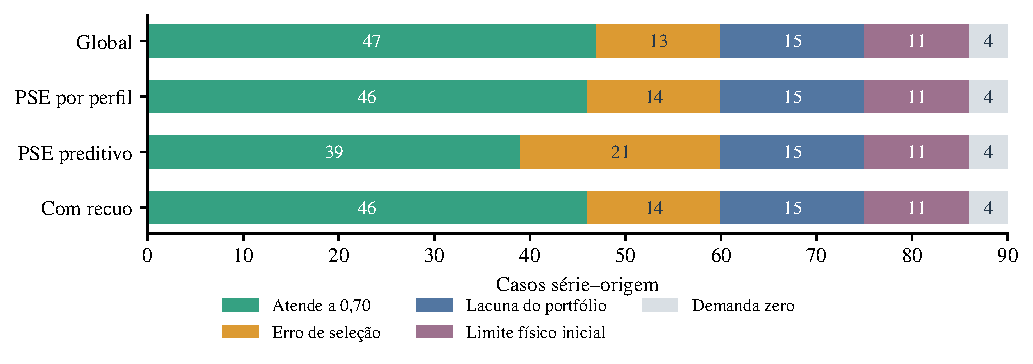
\includegraphics[width=.97\linewidth]{figures/aipe_m5_falhas.pdf}
\caption{Decomposição dos 90 casos M5. Erro de seleção: outra candidata atende. Lacuna do portfólio: nenhuma candidata atende, mas o planejamento perfeito permite atender. Limite físico: condições iniciais impedem atingir 0,70. Demanda zero mantém serviço indefinido.}\label{fig:m5_failure}
\end{figure}

No preditivo, 39 casos atendem ao alvo; 21 falham apesar de existir política viável; 15 falham sem candidata viável, embora o planejamento perfeito permita atender; 11 têm restrição física inicial; e quatro têm demanda zero. O recuo reduz os erros de seleção de 21 para 14. Melhorar o seletor não resolve sozinho todas as faltas: a Figura~\ref{fig:m5_failure} separa intervenções sobre escolha, controle e abastecimento inicial.
\FloatBarrier

\subsection{Instanciação do PSE por consequências e recuo}
\label{sec:consequencias_compacto}
A substituição do seletor na mesma matriz permite comparar implementações sem refazer os controladores (Tabela~\ref{tab:consequencias_compacto}). A floresta por consequências sem recuo reduz o custo em 0,33\%, mas perde 2,09 pontos de atendimento frente à global. O controle por classe vencedora também reduz custo e perde serviço, limitando atribuir a melhora frente ao XGBoost somente ao alvo de aprendizagem.

\begin{table}[htbp]\centering\small
\caption{Variantes do PSE na mesma matriz M5: 90 casos de custo e 86 de serviço definido. Referências global, por perfil e preditiva por classe constam da Tabela~\ref{tab:m5_selectors}.}\label{tab:consequencias_compacto}
\begin{tabular}{@{}p{5.2cm}rrr@{}}\toprule
Variante & Custo & Serviço & Casos $\geq0{,}70$\\\midrule
Classe vencedora: floresta de controle & 1.074,17 & 68,97\% & 40\\
Consequências sem recuo & 1.083,36 & 69,37\% & 38\\
Consequências sem perfil e sem recuo & 1.148,09 & 69,25\% & 38\\
Consequências com recuo & 1.070,03 & 71,72\% & 47\\\bottomrule
\end{tabular}\end{table}

Com recuo, o custo médio fica 1,56\% abaixo da global e o serviço 0,27 ponto acima (Figura~\ref{fig:consequencias_compacto}). Somente três decisões mudam: uma de CappedBaseStock para GA em CA\_2 e duas de EOQCycle para sSCycle em TX\_2. Uma série concentra aproximadamente 92\% da economia. Duas intervenções permanecem abaixo de 70\% apesar de viabilidade prevista. São mantidos os mesmos 47 casos que atendem ao alvo, sem novas falhas ou recuperações frente à global.

\begin{figure}[htbp]\centering
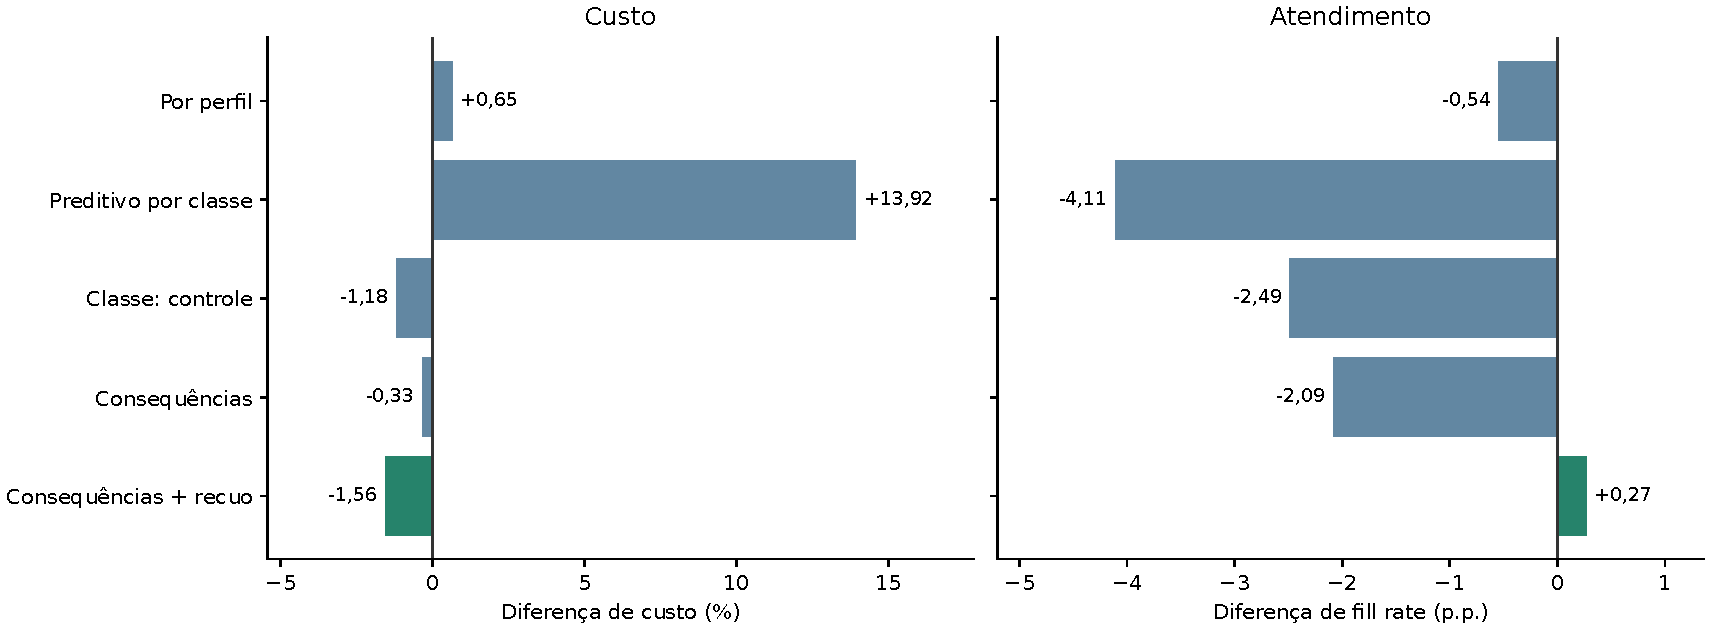
\includegraphics[width=\linewidth]{figures/aipe_consequencias_comparacao.pdf}
\caption{Diferenças médias frente à global. O recuo limita intervenções, mas o benefício observado concentra-se em duas lojas e não demonstra transferência.}\label{fig:consequencias_compacto}
\end{figure}

Intervalos exploratórios de 95\%, por bootstrap pareado de dez lojas, são $[-48{,}10;0{,}00]$ para diferença de custo e $[0{,}000;0{,}734]$ ponto para serviço. Alcançam zero, condicionam-se aos ajustes fixos e não corrigem multiplicidade. A comparação favorece investigar intervenção seletiva, com confirmação em dados que não tenham orientado essa revisão.


\section{Discussão}
Os resultados distinguem a viabilidade de executar o AIPE do benefício de contextualizar a reposição. Controladores e seletores distintos operam sob os contratos definidos, exercitando a modularidade do procedimento. Seu valor operacional depende de uma segunda verificação: a recomendação precisa melhorar o compromisso entre custo e atendimento frente a uma referência competitiva. A execução de alternativas, por si só, não estabelece esse benefício.

Na Bahia, a seleção por perfil acrescenta atendimento com custo pontualmente maior; na segunda origem, coincide com a escolha global. Esse comportamento mostra que a utilidade da segmentação depende da janela e do critério operacional. A base brasileira fortalece a relevância aplicada da avaliação ao preservar heterogeneidade observada em vendas empresariais, enquanto a simulação e a possível censura por ruptura delimitam a interpretação econômica.

O piloto M5 evidencia a dificuldade de aprender a identidade da melhor família com pouco suporte. O XGBoost perde para a referência em custo e atendimento. A previsão de consequências preserva a magnitude operacional dos erros de escolha, mas sua implementação direta também perde serviço; o controle por classe com outra floresta altera os resultados. Portanto, a comparação não isola todo o efeito do alvo de aprendizagem.

O recuo à global restringe a intervenção e concentra a investigação nas decisões em que o seletor prevê uma vantagem. A variante por consequências conserva a referência em 87/90 casos, melhora pontualmente custo e serviço e concentra cerca de 92\% da economia em uma série. Esse padrão sustenta a investigação de intervenções seletivas, com análise de concentração e deteriorações. Seu desenvolvimento no mesmo piloto impede interpretá-lo como confirmação independente da melhoria.

Os oráculos mostram que corrigir o seletor é apenas uma das intervenções possíveis. Havendo candidata viável, a escolha pode ser aprimorada; sem candidata viável, deve-se examinar o portfólio e sua calibração; diante de inviabilidade física, é necessário rever as condições do sistema. A distinção orienta qual componente do AIPE merece revisão e evita atribuir toda ruptura ao modelo preditivo.

O suporte do contexto também limita a transferência. Na primeira origem M5, 826/885 séries elegíveis são esparsas, 57 têm tendência e duas pertencem ao grupo volatilidade/sazonalidade. Mais séries não asseguram diversidade de perfis. A ampliação precisa preservar a definição do serviço: meta média, atendimento ponderado e garantia por série respondem a objetivos distintos. Alterar um módulo exige manter esse significado e conferir novamente as consequências.

\section{Limitações e próximos testes}
Vendas podem omitir demanda censurada por falta. Coortes históricas, elegibilidade na primeira origem e horizontes de sete ciclos restringem população e período. Produtos compartilhados entre lojas podem gerar dependência não capturada inteiramente pelo bootstrap.

Não se trata de experimento causal de implantação. Custos não são financeiramente calibrados, não há suprimento conjunto e o estado inicial comum não reproduz trajetórias particulares. A calibração distinta da CappedBaseStock e os esforços desiguais limitam comparações entre algoritmos e bases.

As extensões com recuo foram desenvolvidas no piloto; suas métricas não confirmam independentemente a melhoria. A substituição foi exercitada nas candidatas e no PSE, sem ablação de todas as representações e ambientes. Assim, a portabilidade integral permanece uma hipótese de uso. A avaliação ampliada precisa examinar suporte por perfil e classe, restrições de serviço comparáveis e validação interna por loja para ajustes do seletor. Séries reservadas devem ficar fora dessas decisões. Harmonização da calibração e sensibilidades de custo, prazo e horizonte precedem conclusões mais amplas.

\section{Conclusão}
O AIPE propõe um procedimento modular para escolher políticas de reposição conforme o contexto da série loja--produto. Sua contribuição articula evidência comparável, duas abordagens do PSE, uma decisão explícita de intervenção e diagnóstico das perdas. Os métodos utilizados preenchem essas responsabilidades e permitem avaliar escolhas alternativas sem redefinir todo o problema.

A avaliação delimita onde essas escolhas ajudam. Na Bahia, o perfil acrescenta 3,89 pontos de atendimento com aumento de custo de 1,93\%. No piloto M5, a estimação por classe perde para a global; consequências com recuo reduzem custo em 1,56\% e acrescentam 0,27 ponto de atendimento, com apenas três intervenções e benefício concentrado. Assim, a evidência sustenta a execução e a utilidade diagnóstica do procedimento, enquanto seu benefício operacional permanece condicionado à instanciação.

A confirmação requer calibrações harmonizadas e avaliação da regra de intervenção em dados reservados, excluídos do desenvolvimento. O critério decisivo será a capacidade de reconhecer quando uma recomendação contextual compensa e quando preservar a referência, considerando serviço, custo e deteriorações.

\section*{Disponibilidade de dados e código}
Os dados brasileiros são proprietários e não são redistribuídos; o M5 é público. Código, configurações e fontes estão em \url{https://github.com/matheus013/msc}. Dados, bancos e modelos ficam fora da versão atual do repositório. Manifestos e snapshots locais identificam as matrizes; pacote arquivado e derivados autorizados deverão acompanhar a submissão. Não se promete acesso aos registros restritos mediante solicitação.

\section*{Autoria, financiamento e interesses}
Autoria, contribuições dos autores, financiamento, agradecimentos e interesses devem ser confirmados pelos autores responsáveis. O manuscrito em português requer tradução, revisão humana e fechamento das declarações antes da submissão.

\section*{Uso de inteligência artificial na preparação do manuscrito}
OpenAI Codex auxiliou organização bibliográfica, leitura de código, análise, visualização e redação. A figura conceitual usa desenhos vetoriais programáticos; os gráficos quantitativos derivam das matrizes identificadas. Conferência e responsabilidade pelo texto final cabem aos autores humanos. Sistemas de inteligência artificial não são autores.

\bibliographystyle{elsarticle-num}
\bibliography{references_ptbr}
\end{document}
